\chapter{推し活の便益と負担に関する質問紙調査（RQ1）}
本章では，RQ1「性格特性（TIPI-J）と推し活行動は，幸福度・推し疲れとどのように関連し，個人の見込みとしてどの程度の精度で予測できるか」に答えるために行った質問紙調査について述べる．調査の目的，対象と手続き，測定項目，分析方法，結果を順に述べ，最後に結果から導いたシステムの設計指針を示す．

\section{調査の目的}
本調査の目的は次の3点である．
\begin{enumerate}
\item 推し活の便益（幸福度）と負担（推し疲れ）がどの程度同時に生じているか，またそれらがどの行動から生じているかを明らかにする（RQ1a）．
\item 性格特性が推し活の関わり方とどう関連し，行動の効果を調整するかどうかを明らかにする（RQ1b）．
\item 性格・行動・きっかけから，個人の幸福度と推し疲れをどの程度の精度で予測できるかを明らかにする（RQ1c）．
\end{enumerate}
これらの結果は，第4章で述べるOshiFitの提案の仕組みと見込みの示し方の根拠となる．

\section{調査対象と手続き}
推し活を行う日本のファンを対象に，オンラインの質問紙調査を行った．回答者は主に大学の連絡網を通じて募集した．\todo{要記入：調査期間，募集方法の詳細，謝礼の有無，倫理審査の承認番号（2024-26）}回答は匿名で収集し，回答の開始前に研究の目的と回答の任意性を説明した．

回答者は234名であった．このうち，推し活をしていないと回答した17名と，注意確認項目（「この質問には必ず『2 ほとんど当てはまらない』を選んでください」）に誤答した2名を除外し，215名を分析対象とした．分析対象者の内訳は，男性113名，女性94名，その他または無回答8名であり，年齢の中央値は19歳（四分位範囲18〜21歳）であった．

\section{測定項目}
\subsection{性格特性（TIPI-J）}
性格特性の測定には，日本語版Ten Item Personality Inventory（TIPI-J）\cite{oshio2012}の10項目を用いた．原版\cite{gosling2003}および日本語版は7件法であるが，本研究では回答の負担と他の項目との一貫性を考慮して5件法（1：全く違うと思う〜5：強くそう思う）で尋ねた．各因子の得点は，順方向の項目と逆転項目の2項目の平均とした（外向性，協調性，誠実性，神経症傾向，開放性）．2項目からなる尺度は内的一貫性が低くなりやすいことが知られており\cite{gosling2003,oshio2012}，本研究でもその点に留意して解釈する．

\subsection{推し活の行動・没入・きっかけ}
推し活の行動として，推しに関する音楽の聴取，動画の視聴，ライブやイベントへの現地参加，CD・Blu-rayやグッズの購入，テレビ・ラジオのチェック，雑誌・書籍の購入，SNSでの情報収集と発信，聖地巡礼，ファンクラブへの入会，コラボカフェへの来店などの頻度を尋ねた．分析では，視聴，現地イベント，グッズ購入，SNSの4項目を「推し活の頻度」として用いた．

推し活への没入として，推しやキャラクターの世界に入り込む程度を3項目で尋ねた．また，推し活をしたくなるきっかけとして，「仕事や学校などで嫌なことがあり，ストレスから逃れたいとき」（逃避），「何かを頑張った後の，自分へのご褒美として」（ご褒美），「疲れているとき，癒やしや元気をもらいたいとき」（回復）の3項目を「気分の回復のための推し活」として用いた．

\subsection{幸福度と推し疲れ}
推し活による幸福度（便益）は，推し活を通じた生活の張り（毎日の生きがい），スケジュール管理，自分への自信，創作スキルの向上の4項目で測定した．推し疲れ（負担）は，睡眠への支障，お金の不安，義務感，SNS上での他のファンへの嫉妬の4項目で測定した．いずれも本研究のために構成した推し活固有の合成得点である．

\subsection{回答のコーディング}
回答データは，回答フォームの仕様により「1」が最も強い同意または最も高い頻度を表す形で保存されていた（例：動画視聴の素点の平均は1.25，現地イベントは3.99）．そこで，すべての項目を「数値が大きいほど多い・強い」向きになるよう逆転し，質問紙の原本と照合してこの処理が正しいことを確認した．なお，中間の選択肢（「どちらでもない」）の選ばれやすさは回答者の動機づけや項目数の影響を受けることが知られているため\cite{masuda2014}，注意確認項目による除外を行った．

表\ref{tab:measures}に，分析に用いた構成概念と，その信頼性係数（Cronbachの$\alpha$），平均値，標準偏差を示す．

\begin{table}[t]
\centering
\jetcaption{分析に用いた構成概念（$N=215$，1〜5点，高いほど多い・強い）}{Measures ($N=215$; 1--5, higher = more)}
\label{tab:measures}
\small
\begin{tabular}{@{}p{0.55\linewidth}ccc@{}}
\toprule
構成概念（項目数） & $\alpha$ & 平均 & 標準偏差 \\
\midrule
推し活の頻度（視聴，現地イベント，グッズ，SNS；4） & .43 & 3.32 & 0.58 \\
推し活への没入（3） & .62 & 3.51 & 0.96 \\
気分の回復のための推し活（逃避，ご褒美，回復；3） & .58 & 4.07 & 0.88 \\
幸福度（生きがい，スケジュール管理，自信，創作；4） & .57 & 3.23 & 0.83 \\
推し疲れ（睡眠，お金，義務感，嫉妬；4） & .70 & 2.38 & 0.97 \\
\bottomrule
\end{tabular}
\end{table}

\section{分析方法}
本節の分析方法（類型化，パスモデル，調整効果の検定，予測精度の推定，補助的な因果分析）は，指導教員の大井翔講師に加え，データサイエンス学科の濱田悦夫教授から統計解析に関する助言を得て決定した．

\subsection{行動パターンの類型化}
推し活の行動パターンを把握するため，標準化した推し活の頻度に対してk-means法によるクラスタリングを行った．クラスタ数$k$は2〜8の範囲で試し，各$k$について初期値を変えて50回実行した．クラスタ数はシルエット係数\cite{rousseeuw1987}が最大となるものを選んだ．得られた群の間で幸福度と推し疲れを比較し，Welchの$t$検定とCohenの$d$で差の大きさを評価した．

\subsection{パスモデル}
性格・推し活の関わり方・幸福度と推し疲れの関係を検討するため，観測変数によるパスモデル（構造方程式モデリング\cite{toyoda1998}）を推定した．性格特性の5因子が推し活の頻度・没入・気分の回復のための推し活を予測し，これら8変数すべてが幸福度と推し疲れを予測するモデルとした．推定にはPythonのsemopy\cite{igolkina2020}を用い，最尤法で推定した標準化係数を報告する．このモデルはほぼ飽和しているため，適合度ではなく係数の大きさと向きを解釈する．なお，横断的なデータであるため，矢印の向きは仮定した方向を表すものであり，因果関係を示すものではない．

\subsection{性格による調整効果}
性格特性が推し活の頻度の効果を調整するかどうかを検討するため，幸福度と推し疲れをそれぞれ目的変数とする回帰モデルに，推し活の頻度と性格5因子の交互作用項を加え，交互作用項を含まないモデルと入れ子の$F$検定で比較した．また，性格特性のみによるクラスタリングも行い，性格による「タイプ」の分離のよさをシルエット係数で評価した．

\subsection{プロファイルと理想}
幸福度と推し疲れのそれぞれの中央値で回答者を分け，4つのプロファイル（両方高い，充実型，負担型，控えめ型）に分類した．また，各活動について「理想の頻度」から「現在の頻度」を引いた値の符号を求め，増やしたい・減らしたい活動を集計した．

\subsection{予測精度}
個人の幸福度と推し疲れをどの程度の精度で予測できるかを評価するため，性格・推し活の頻度・没入・きっかけを説明変数とする線形の予測モデルを作り，10分割交差検証によって決定係数（$R^2$）と平方根平均二乗誤差（RMSE）を推定した．

\subsection{補助的な分析}
本研究では，パスモデルで仮定した矢印の向きがデータから支持されるかを確かめるために，時間の順序（性格→行動→充実・負担→幸福度）を背景知識として与えたPCアルゴリズム\cite{spirtes2000}による因果構造の探索と，ほかの行動や性格・きっかけを調整したうえで各行動が推し疲れ・幸福度に与える効果を推定するDouble Machine Learning（DML）\cite{chernozhukov2018}も行った．複数の手法で同じ向きが得られた行動だけを提案の根拠に用いる（三角測量）．\todo{要記入：PCアルゴリズムとDMLの結果（推定された向き，効果量と信頼区間）}

\section{結果}
\subsection{便益と負担の共存}
回答者の79\%が推しは「生きがい」を与えてくれると回答した．一方で，40\%がお金の不安，33\%が睡眠への支障，20\%がSNS上での嫉妬，14\%が義務感を報告した．幸福度と推し疲れの間には正の相関が見られた（$r=.24$）．すなわち，推し活によって幸福を感じている人ほど，推し疲れも感じやすい傾向があった．

\subsection{行動パターン}
k-meansによるクラスタリングでは$k=2$のときにシルエット係数が最大（0.41）となり，日常的にSNSを中心に推し活を行う群（166名）と，視聴を中心に推し活を行う群（49名）に分かれた．SNS中心の群は視聴中心の群に比べて幸福度が大きく高かった（3.39対2.67，$d=0.94$，$p<.001$）が，推し疲れはやや高い程度であった（2.45対2.14，$d=0.32$，$p=.07$）．

\subsection{RQ1a：同じ行動が便益と負担の両方を生む}
図\ref{fig:paths}と表\ref{tab:paths}に，パスモデルの結果を示す．推し活の頻度は，幸福度の高さ（$\beta=.43$）と推し疲れの高さ（$\beta=.29$）の両方と関連した．推し活への没入も同様に，幸福度（$\beta=.20$）と推し疲れ（$\beta=.23$）の両方と関連した（いずれも$p<.001$）．一方，気分の回復のための推し活は幸福度とのみ関連し（$\beta=.18$，$p=.003$），推し疲れとは関連しなかった（$p=.47$）．決定係数は幸福度で.34，推し疲れで.20であった．

\begin{figure}[t]
\centering
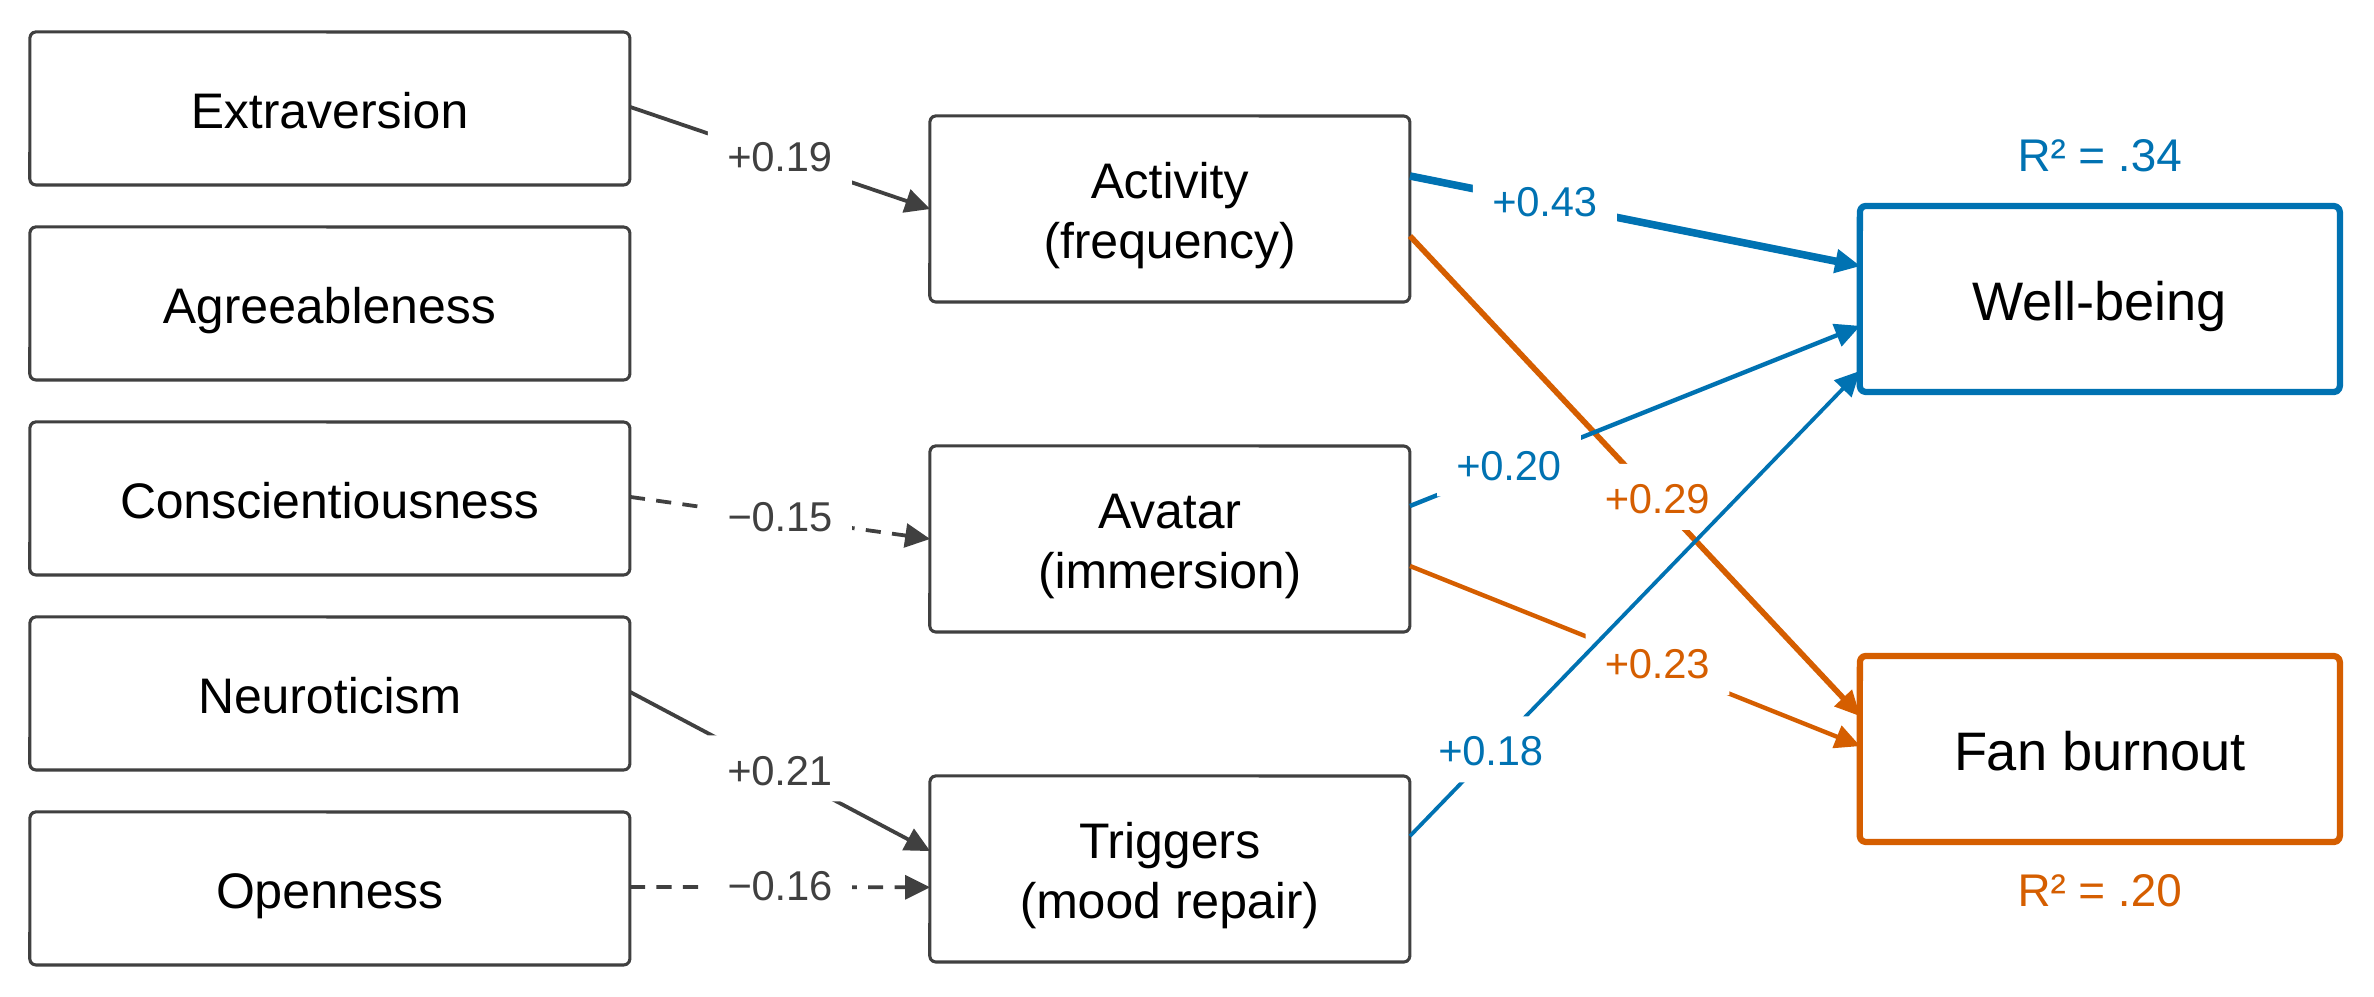
\includegraphics[width=0.85\linewidth]{figures/fig3_paths_ppt.png}
\jecaption{パスモデルの結果（$N=215$，標準化係数，$p<.05$のみ表示，破線は負の関係．青は幸福度へ，橙は推し疲れへの経路．協調性には有意な経路がなかった）}{Path model ($N=215$; standardised, $p<.05$ only; dashed = negative)}
\label{fig:paths}
\end{figure}

\begin{table}[t]
\centering
\jetcaption{パスモデルの主な標準化係数}{Main standardised coefficients of the path model}
\label{tab:paths}
\small
\begin{tabular}{@{}llrl@{}}
\toprule
説明変数 & 目的変数 & $\beta$ & 有意性 \\
\midrule
推し活の頻度 & 幸福度 & .43 & $p<.001$ \\
推し活の頻度 & 推し疲れ & .29 & $p<.001$ \\
推し活への没入 & 幸福度 & .20 & $p<.001$ \\
推し活への没入 & 推し疲れ & .23 & $p<.001$ \\
気分の回復のための推し活 & 幸福度 & .18 & $p=.003$ \\
気分の回復のための推し活 & 推し疲れ & -- & $p=.47$（n.s.） \\
\midrule
外向性 & 推し活の頻度 & .19 & $p<.05$ \\
誠実性 & 推し活への没入 & $-.15$ & $p<.05$ \\
神経症傾向 & 気分の回復のための推し活 & .21 & $p<.05$ \\
開放性 & 気分の回復のための推し活 & $-.16$ & $p<.05$ \\
\midrule
\multicolumn{4}{@{}l}{決定係数：幸福度 $R^2=.34$，推し疲れ $R^2=.20$} \\
\bottomrule
\end{tabular}
\end{table}

\subsection{RQ1b：性格は推し活の関わり方を形づくる}
性格特性は，推し活の関わり方と関連した．外向性は推し活の頻度の高さと（$\beta=.19$），誠実性は没入の低さと（$\beta=-.15$），神経症傾向は気分の回復のための推し活の多さと（$\beta=.21$），開放性はその少なさと（$\beta=-.16$）関連した．ただし，これらの効果はいずれも小さかった（$|\beta|\leq.21$）．協調性は，どの変数とも有意な関連を示さなかった．

推し活の頻度と性格5因子の交互作用項を加えても，決定係数はほとんど変化しなかった（幸福度：.344→.353，$p=.74$；推し疲れ：.196→.205，$p=.79$）．すなわち，推し活の頻度が幸福度や推し疲れに与える効果は，性格によって大きく変わるわけではなかった．

また，性格特性のみによるクラスタリングでは，シルエット係数が0.15〜0.18と低く，明確な「タイプ」には分かれなかった．3群の解では，群の間で推し疲れにわずかな差が見られた（$\eta^2=.04$，$p=.01$）．以上から，性格は単独の「タイプ」として提案に用いるよりも，行動と組み合わせて用いるのが適切であると考えられる．

\subsection{プロファイルと理想}
幸福度と推し疲れの中央値で分けた4つのプロファイルの割合を表\ref{tab:profiles}に示す．両方高い人が27\%，幸福度が高く推し疲れが低い充実型が22\%，幸福度が低く推し疲れが高い負担型が21\%，両方低い控えめ型が31\%であった．

\begin{table}[t]
\centering
\jetcaption{幸福度と推し疲れによる4つのプロファイル}{Four profiles by well-being and burnout}
\label{tab:profiles}
\small
\begin{tabular}{@{}llll@{}}
\toprule
プロファイル & 幸福度 & 推し疲れ & 割合 \\
\midrule
両方高い & 高い & 高い & 27\% \\
充実型 & 高い & 低い & 22\% \\
負担型 & 低い & 高い & 21\% \\
控えめ型 & 低い & 低い & 31\% \\
\bottomrule
\end{tabular}
\end{table}

理想と現在の頻度の差を見ると，39\%が現地イベントを，36\%がグッズの購入を「増やしたい」と回答し，「減らしたい」と回答したのはそれぞれ1\%と5\%にとどまった．最も多く「減らしたい」と回答された活動はSNSであった（22\%）．すなわち，多くのファンは推し活を全体として減らしたいわけではなく，増やしたい活動と整えたい活動が混在していた．

\subsection{RQ1c：個人の予測の精度}
性格・行動・きっかけを組み合わせた線形の予測モデルの交差検証決定係数は，幸福度で.27（RMSE 0.71），推し疲れで.11（RMSE 0.92）であった．また，ある1つの活動の頻度を1段階変えたときの予測値の変化は0.1〜0.2点にとどまり，予測の誤差よりも小さかった．すなわち，個人の幸福度と推し疲れの予測には大きな不確かさが伴う．

\section{考察}
本調査の結果，推し活の便益と負担は同じ行動（頻度と没入）から生じていることが示された．このことは，推し活に対して一律に「減らす」助言を行うと，負担だけでなく幸福度も下げてしまう可能性が高いことを意味する．また，多くのファンが現地イベントやグッズを増やしたいと考えている一方で，SNSについては減らしたいと考える人が一定数いたことから，推し活全体ではなく，本人にとって負担となっている特定の関わり方（例えば，深夜のSNS閲覧や他のファンとの比較）を整えることが支援の方向性として適切であると考えられる．

性格特性は，推し活の関わり方（どのくらい活動するか，どのくらい没入するか，気分の回復のために推し活をするか）と関連していたが，行動の効果を調整していなかった．また，性格だけでは明確なタイプに分かれなかった．このことから，性格を「あなたは○○タイプだから△△をすべき」という固定的な処方に用いるのではなく，本人の行動や負担の状況と組み合わせ，複数の提案の中から本人に合いやすいものを優先する手がかりとして用いるのが適切である．

予測の精度が限られていたことは，個人の見込みを点の値だけで示すと過信を招くおそれがあることを示している．見込みは幅とともに示し，差が小さい場合には「ほぼ同じ」と伝えるなど，不確かさを正直に示す必要がある．

本調査には限界もある．回答者は大学の連絡網を通じて募集した若年層が中心であり，推し活を行う人全体を代表しているとは限らない．TIPI-Jを5件法で用いたこと，一部の合成得点の信頼性係数が低かったこと（推し活の頻度$\alpha=.43$など）にも留意が必要である．また，横断的な調査であるため，示された関連は因果関係を意味しない．

\section{システムの設計指針}
以上の結果から，次の4つの設計指針を導いた．

\begin{description}
\item[D1：一律に減らす助言をしない．]便益と負担は同じ行動から生じるため，推し活を一律に減らす助言は行わない．「今のまま」を常に有効な選択肢として示す．
\item[D2：性格と行動を組み合わせて個人化する．]性格を固定的なタイプとして扱わず，本人の行動と負担の状況を主な手がかりとし，性格は提案の優先順位を決める補助として用いる．
\item[D3：便益と負担を同時に示す．]幸福度と推し疲れの両方を示し，提案による変化のトレードオフも示す．
\item[D4：不確かさを正直に示す．]見込みは幅とともに示し，得点の算出式と使用項目を開示する．
\end{description}

第4章では，これらの設計指針に基づいて構築したOshiFitについて述べる．
